\begin{center}
	\section{Modelo CFD-DEM} \label{CFD-DEM}
\end{center}

\noindent
\justify

El modelo CFD-DEM consiste de una metodolog\'ia de c\'alculo, a trav\'es de los m\'etodos num\'ericos de vol\'umenes finitos (FVM) y elementos discretos (DEM), que busca predecir el comportamiento din\'amico de las part\'iculas en un medio fluido.

\noindent
\justify

La metodolog\'ia se resume en lo siguiente:

\begin{enumerate}
	\item Definici\'on de la geometr\'ia del problema.
	\item Mallado de la geometr\'ia para el an\'alisis fluidodin\'amico mediante CFD.
	\item Definici\'on de las condiciones de frontera.
	\item Desarrollo de la simulaci\'on CFD - DEM.
	\item Postprocesamiento y presentaci\'on de resultados.
\end{enumerate}

\noindent
\justify

Se desarroll\'o un algoritmo a trav\'es de herramientas de \textit{c\'odigo abierto}: Python como lenguaje base; Jupyter como entorno de desarrollo; OpenFOAM y Yade para el desarrollo las simulaciones num\'ericas; y ParaView como entorno de presentaci\'on de resultados de post-procesamiento.

\subsection{Geometr\'ia} \label{geo}

\noindent
\justify

Para la definici\'on de la geometr\'ia, se desarroll\'o una metodolog\'ia de c\'alculo te\'orico autom\'atico en Python - Jupyter para diferentes problemas de inter\'es, conforme a la metodolog\'ia planteada en el Cap\'itulo \ref{teorico:sed}.

\noindent
\justify

El di\'ametro de la entrada de la mezcla \textit{solvente - material pulverizado} est\'a definido por la Ecuaci\'on \ref{D_I}.

\begin{equation}
	D_I = \frac{4 Q_T}{Re \, \pi \mu}
	\label{D_I}
\end{equation}

\noindent
\justify

En d\'onde: $D_I$ es el di\'ametro de ingreso de la mezcla s\'olido - l\'iquido, $Q_T$ es el caudal del problema, $Re$ es el n\'umero de Reynolds y $\mu$ es la viscosidad cinem\'atica del fluido.

\noindent
\justify

Con base en los resultados mostrados en el Cuadro \ref{resul_dis}, el di\'ametro de ingreso tiene un valor de $27 [cm]$. La geometr\'ia con la que se desarrolla el presente modelo se puede apreciar en la Figura \ref{geometria:CFD}.



\newpage

\noindent
\justify

De la Figura \ref{geometria:CFD}, el \'area sombreada corresponde a la geometr\'ia de an\'alisis, en donde se observa: una zona de \textit{entrada} de la mezcla s\'olido - l\'iquido; una de \textit{salida} (al final de la superficie inclinada), en donde se espera obtener la \textit{fase l\'iquida} de la mezcla; y un \'area de dep\'osito de lodos, localizada en la parte inferior de la geometr\'ia, en donde se deposita el material particulado.

\subsection{Mallado}

\noindent
\justify

Gran parte del \'exito de las simulaciones num\'ericas recaen en la discretizaci\'on del dominio y en la calidad de los elementos que la componen$^{\cite{Roda-Casanova2021}}$. Se desarroll\'o una metodolog\'ia de mallado autom\'atico con base en el lenguaje \textit{gmsh} tomando como variables de entrada las dimensiones de la geometr\'ia definida en la secci\'on \ref{geo}. Esta metodolog\'ia emplea elementos de diferentes tama\~nos y permite tambi\'en definir su naturaleza (rectangulares o triangulares).

\noindent
\justify

El algoritmo ejecuta, adem\'as, un refinamiento autom\'atico en la zona en donde ocurre el mayor grado de sedimentaci\'on: en la superficie inclinada, como se aprecia en la Figura \ref{malla:geo}.

\begin{figure}[h!]
	\centering
	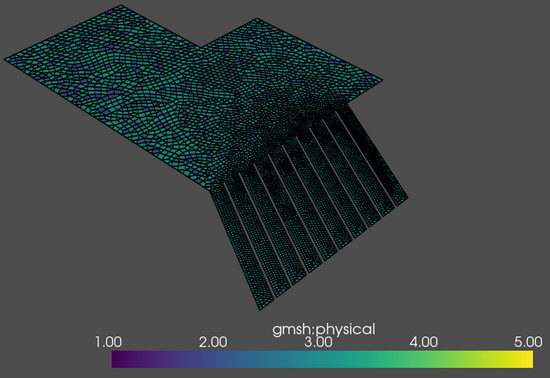
\includegraphics[width=\textwidth]{Images/CFDEM/malla2.png}
	\caption{Mallado de la geometr\'ia.}
	\label{malla:geo}
\end{figure}

\newpage

\noindent
\justify

La malla mostrada en la Figura \ref{malla:geo} presenta las siguientes caracter\'isticas:

\begin{table}[h!]
	\centering
	\begin{tabular}{|c|c|}
		\hline
		\textbf{Par\'ametro} & \textbf{Valor} \\ \hline
		Tipo de elementos & Rectangulares \\ \hline
		N\'umero de elementos & 20415 \\ \hline
		N\'umero de nodos & 13692 \\ \hline	
	\end{tabular}
	\caption{Datos de la malla generada.}
	\label{malla}
\end{table}

\noindent
\justify

Al emplear el m\'etodo \texttt{checkMesh} de OpenFOAM para el an\'alisis preliminar de malla, se obtuvieron los siguientes resultados:

\begin{table}[h!]
	\centering
	\begin{tabular}{|c|c|}
		\hline
		\textbf{Par\'ametro} & \textbf{Valor} \\ \hline
		Apertura \textit{m\'axima} entre elementos & 11.45 \\ \hline
		Checkeo de \textit{no} ortogonalidad & OK \\ \hline
		Oblicuidad m\'axima & 0.66 OK \\ \hline
		Conclusi\'on de malla & OK \\ \hline
	\end{tabular}
	\caption{Resumen de resultados sobre el checkeo de malla.}
	\label{check}
\end{table}

\noindent
\justify

A partir de los resultados mostrados en el Cuadro \ref{check}, se concluye que la malla es \'optima para el desarrollo de las simulaciones num\'ericas consecutivas.

\newpage

\subsection{Desarrollo de la simulaci\'on}

\noindent
\justify

La simulaci\'on num\'erica a realizar comprende \textbf{dos} m\'etodos num\'ericos: el m\'etodo de \textit{vol\'umenes finitos} (FVM, por sus siglas en ingl\'es), con el cual se predice el comportamiento fluidodin\'amico dentro del volumen de control, y el m\'etodo de \textit{elementos discretos} (DEM, por sus siglas en ingl\'es) con el que se predice el comportamiento din\'amico de las part\'iculas s\'olidas y su interacci\'on con el solvente.

\subsubsection{CFD} \label{CFD:problema}

\noindent
\justify

La \textit{Din\'amica de Fluidos Computacional} (CFD) es una herramienta ampliamente usada en ingenier\'ia para el desarrollo de simulaciones num\'ericas que involucren fluidos. Emplea como m\'etodo base el m\'etodo de vol\'umenes finitos (FVM). Este m\'etodo num\'erico transforma las ecuaciones diferenciales parciales, que representan las leyes conservativas, en ecuaciones algebraicas discretas sobre vol\'umenes finitos.

\noindent
\justify

Desde un punto de vista de \textit{mec\'anica de fluidos computacional}, el presente problema busca estudiar un flujo con las siguientes caracter\'isticas:

\begin{itemize}
	\item Laminar.
	\item Incompresible.
	\item Transitorio.
	\item Fluido newtoniano.
\end{itemize}

\noindent
\justify

Trat\'andose, adem\'as, de un problema \textit{bidimensional}, que matem\'aticamente hablando se refiere a lo siguiente:

\begin{equation}
    \underbrace{\rho \frac{\partial \phi}{\partial t}}_{\text{transitorio}} + \underbrace{\rho u \frac{\partial \phi}{\partial x} + \rho v \frac{\partial \phi}{\partial y}}_{\text{convectivo}} = \underbrace{ \frac{\partial}{\partial x} \left( \Gamma \frac{\partial \phi}{\partial x} \right) + \frac{\partial}{\partial y} \left( \Gamma \frac{\partial \phi}{\partial y} \right)}_{\text{difusivo}} + \underbrace{S_{\phi}}_{\text{fuente}}
    \tag{9}
    \label{2D}
\end{equation}

\noindent
\justify

De la gama de solucionadores est\'andar que maneja OpenFOAM, existen dos que pueden resolver el sistema de ecuaciones de la Ecuaci\'on \ref{2D}: \texttt{icoFoam} y \texttt{pimpleFoam}. Para la soluci\'on del modelo CFD-DEM, se seleccion\'o un solucionador basado en \textit{pimpleFoam} debido a que existe la posibilidad de generaci\'on de turbulencia a ciertas velocidades de flujo del sistema en la interacci\'on fluido-part\'icula.

\noindent
\justify

La l\'ogica de soluci\'on detr\'as de \texttt{pimpleFoam} se puede apreciar en la Figura \ref{pimpleLog}.

% Define block styles
\tikzstyle{decision} = [diamond, draw, fill=blue!20, 
       text width=7em, text badly centered, node distance=3cm, inner sep=0pt]
\tikzstyle{block} = [rectangle, draw, fill=blue!20, 
       text width=7em, text centered, rounded corners, minimum height=4em]
\tikzstyle{line} = [draw, -latex']
\tikzstyle{cloud} = [draw, ellipse,fill=red!20, node distance=3cm,
       minimum height=2em]
\tikzstyle{blockTwo} = [rectangle, draw, fill=blue!20, 
       text width=3em, text centered, rounded corners, minimum height=4em]
\tikzstyle{blockConc} = [rectangle, draw, fill=orange!20, 
       text width=7em, text centered, rounded corners, minimum height=4em]

\begin{figure}[h!]
\centering
\begin{adjustbox}{max width = 0.43\textwidth}
\begin{tikzpicture}[node distance = 2cm, auto]
       % Place nodes
       \node [blockTwo] (init) {Inicio};
       \node [cloud, left of=init] (expert) {Datos};
       \node [decision, below of=init] (decide) {?`$t = t_{final}$?};
       \node [blockConc, right of=decide, node distance=4cm] (update) {Fin};
       \node [block, below of=decide, node distance=3cm] (ecu) {$t = t + \Delta t$};
       \node [block, below of=ecu, node distance=2.5cm] (momento) {Resolver ecuaciones de momento};
       \node [block, below of=momento, node distance=2.5cm] (presion) {Resolver ecuaci\'on de presi\'on};
       \node [block, below of=presion, node distance=2.5cm] (vel) {Corregir campo de velocidades};
       \node [block, below of=vel, node distance=2.5cm] (res) {Resolver sistema de ecuaciones};
       
       \draw (-1.58,-16) -- (-2.5,-16) -- (-2.5, -3) -- (-1.58,-3);
       
       %\node [left of=decide, node distance = 2.5cm] (intermedio)
       % Draw edges
       \path [line] (init) -- (decide);
       \path [line] (decide) -- node {s\'i} (update);
       %\path [line] (update) |- (identify);
       \path [line] (decide) -- node {no}(ecu);
       \path [line] (ecu) -- (momento);
       \path [line] (momento) -- (presion);
       \path [line] (presion) -- (vel);
       \path [line] (vel) -- (res);
       \path [line,dashed] (expert) -- (init);
       %\path [line] (res.west) -- (decide.west);
\end{tikzpicture}
\end{adjustbox}
\caption{Solucionador \texttt{pimpleFoam}.}
\label{pimpleLog}
\end{figure}

\newpage

\paragraph{Resultados} \label{CFD:resultados}

\noindent
\justify

Los resultados de la simulaci\'on num\'erica mediante el m\'etodo de \textit{vol\'umenes finitos} se puede apreciar en las Figuras \ref{CFD:vel} y \ref{CFD:p}.

\begin{figure}[h!]
	\centering
	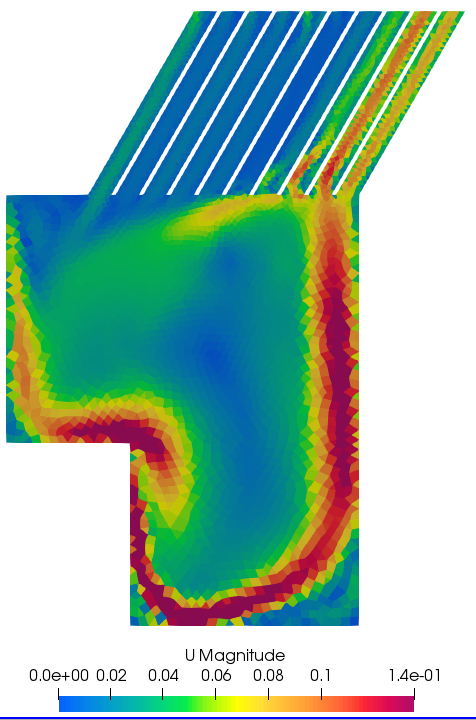
\includegraphics[width=0.35\textwidth]{Images/CFD/vel.png}
	\caption{Diagrama de contorno de la distribuci\'on de velocidades del sistema de sedimentaci\'on.}
	\label{CFD:vel}
\end{figure}

\begin{figure}[h!]
	\centering
	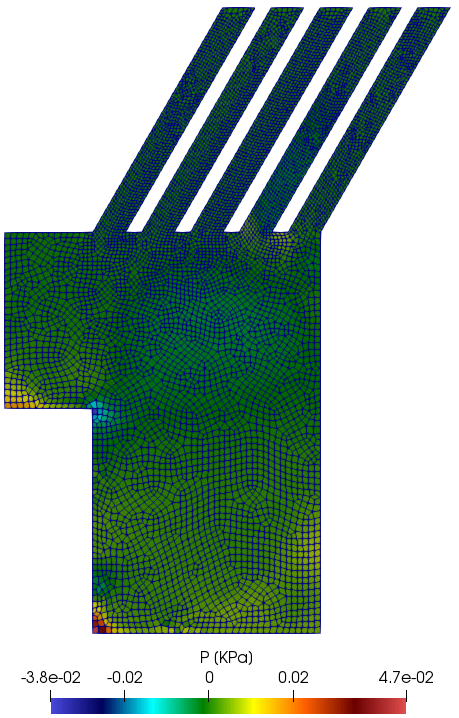
\includegraphics[width=0.35\textwidth]{Images/CFD/p.png}
	\caption{Diagrama de contorno de la distribuci\'on de presiones del sistema de sedimentaci\'on.}
	\label{CFD:p}
\end{figure}

\paragraph{An\'alisis de resultados}

\noindent
\justify

La simulaci\'on num\'erica, desarrollada en OpenFOAM, encontr\'o su punto de equilibrio (punto \textit{estacionario}) al cabo de ocho segundos de simulaci\'on; cuyos resultados, en t\'erminos de velocidad y presi\'on, pueden apreciarse en las Figuras \ref{CFD:vel} y \ref{CFD:p}, respectivamente.

\noindent
\justify

En la Figura \ref{CFD:vel} se observa un valor de velocidad m\'axima de $0.0021 [m/s]$ que es alcanzada en la primera lamela y decrece en las lamelas consecuentes hasta un valor cercano de $0.0015 [m/s]$; fen\'omeno f\'isico que va acorde a la realidad por tratarse de flujos en serie.

\noindent
\justify

En la Figura \ref{CFD:p} se puede apreciar el perfil de presiones sobre el sistema; en donde se presenta un comportamiento uniforme y sim\'etrico alcanzando un valor de presi\'on m\'axima de hasta $0.000012 [kPa]$. Como era de esperarse, las condiciones de frontera establecidas en la secci\'on \ref{CondF} fueron respetadas: en la salida del flujo se aprecia una presi\'on de $0$ (atmosf\'erica) y la velocidad de flujo en la entrada es de $0.00097 [m/s]$.

\subsubsection{CFD-DEM}

\noindent
\justify

El acoplamiento entre CFD \textit{(``Computational Fluid Dynamics")} y DEM \textit{(``Discrete Element Method")} busca predecir la interacci\'on fluido-part\'icula. El flujo se resuelve a trav\'es de CFD basado en malla (ver secci\'on \ref{CFD:problema}), mientras que la fase s\'olida es modelada mediante DEM para cada part\'icula sujeta a trav\'es de fuerzas hidrodin\'amicas, fuerzas de cuerpo (como la gravedad) y a trav\'es de fuerzas de contacto; actualizando valores de velocidad y posici\'on conforme a la segunda ley de Newton (Hoomans \textit{et al.}, 1996; Tsuji \textit{et al.}, 1993; Xu y Yu, 1997). 

\noindent
\justify

La tasa de part\'iculas debido a la sedimentaci\'on, a trav\'es de canales inclinados, ha sido ampliamente estudiado debido al reconocido \textit{efecto Boycott}$^{\cite{Boycott}}$. Este fen\'omeno se produce por el incremento en el \'area efectiva de sedimentaci\'on debido a la presencia de placas inclinadas$^{\cite{Boycott2}}$. Acrivos \textit{et al.} han desarrollado una serie de planteamientos te\'oricos y experimentales entre la tasa de sedimentaci\'on de part\'iculas y el \'area efectiva de sedimentaci\'on. El efecto Boycott ha sido aplicado con \'exito en diversos procesos industriales para la remoci\'on de part\'iculas en lecho de fluidizado a trav\'es del asentamiento gravitacional; entre los principales ejemplos de este hecho se encuentran: tratamientos de aguas residuales$^{\cite{aguares}}$ y procesos de filtrado de agua$^{\cite{aguafil}}$.

\noindent
\justify

El acercamiento experimental para la investigaci\'on caracter\'istica de part\'iculas en suspenci\'on a alta concentraci\'on ha demostrado ser una experiencia retadora debido a las limitantes instrumentales y t\'ecnicas de medici\'on$^{\cite{articulo}}$. Los modelos num\'ericos basados en CFD han demostrado ser una herramienta poderosa y promisoria que provee informaci\'on detallada y precisa sobre las caracter\'isticas locales del flujo particulado. Normalmente, se han aplicado dos enfoques generales en la literatura para resolver problemas que involucran flujo particulado: \textit{Eulerian - Eulerian} (E-E) y \textit{Eulerian - Lagrange} (E-L). En el enfoque E-E, las fases s\'olida y el fluida son interpretadas de manera continua en donde comparten el mismo gripo de ecuaciones gobernantes. Doroodchi \textit{et al.}$^{\cite{ref1}}$ emplearon el modelo E-E para investigar la influencia de las placas inclinadas y el efecto expansivo de s\'olidos en suspensi\'on en camas de lecho fluidizado; obteniendo resultados prometedores tanto en la parte experimental como num\'erica. Salem \textit{et al} $^{\cite{ref2}}$ desarrollaron un modelamiento en CFD empleando el modelo E-E para evaluar las caracter\'isticas hidr\'aulicas de un sedimentador de placas hidr\'aulicas (IPS, por sus siglas en ingl\'es); demostrando que el importante rol que cumplen las herramientas computacionales en el estudio de los sistemas de sedimentaci\'on. Sin embargo, el tratamiento de la fase s\'olida de manera continua va en contra de la naturaleza discreta de las part\'iculas s\'olidas, y todav\'ia m\'as importante: el acercamiento a trav\'es de E-E carece de facultades num\'ericas para revelar informaci\'on importante referente a la escala particular.

\noindent
\justify

El enfoque otorgado por el modelo E-L, por otro lado, adopta la teor\'ia continua para la fase l\'iquida y resuelve el problema cinem\'atico de cada part\'icula individual \textbf{directamente}. Informaci\'on 



